\label{sec:sqrt3}

This scheme was introduced as an adaptive scheme~\cite{sqrt3}, but we
restrict our example program to a single uniform subdivision step, see
Fig.~\ref{fig:sqrt3} for an example of a subdivision sequence and
Fig.~\ref{fig:sqrt3_basic} for a closeup on the refinement.

% sqrt3 subdivision (basic)

\begin{figure}[htb]
    \centering{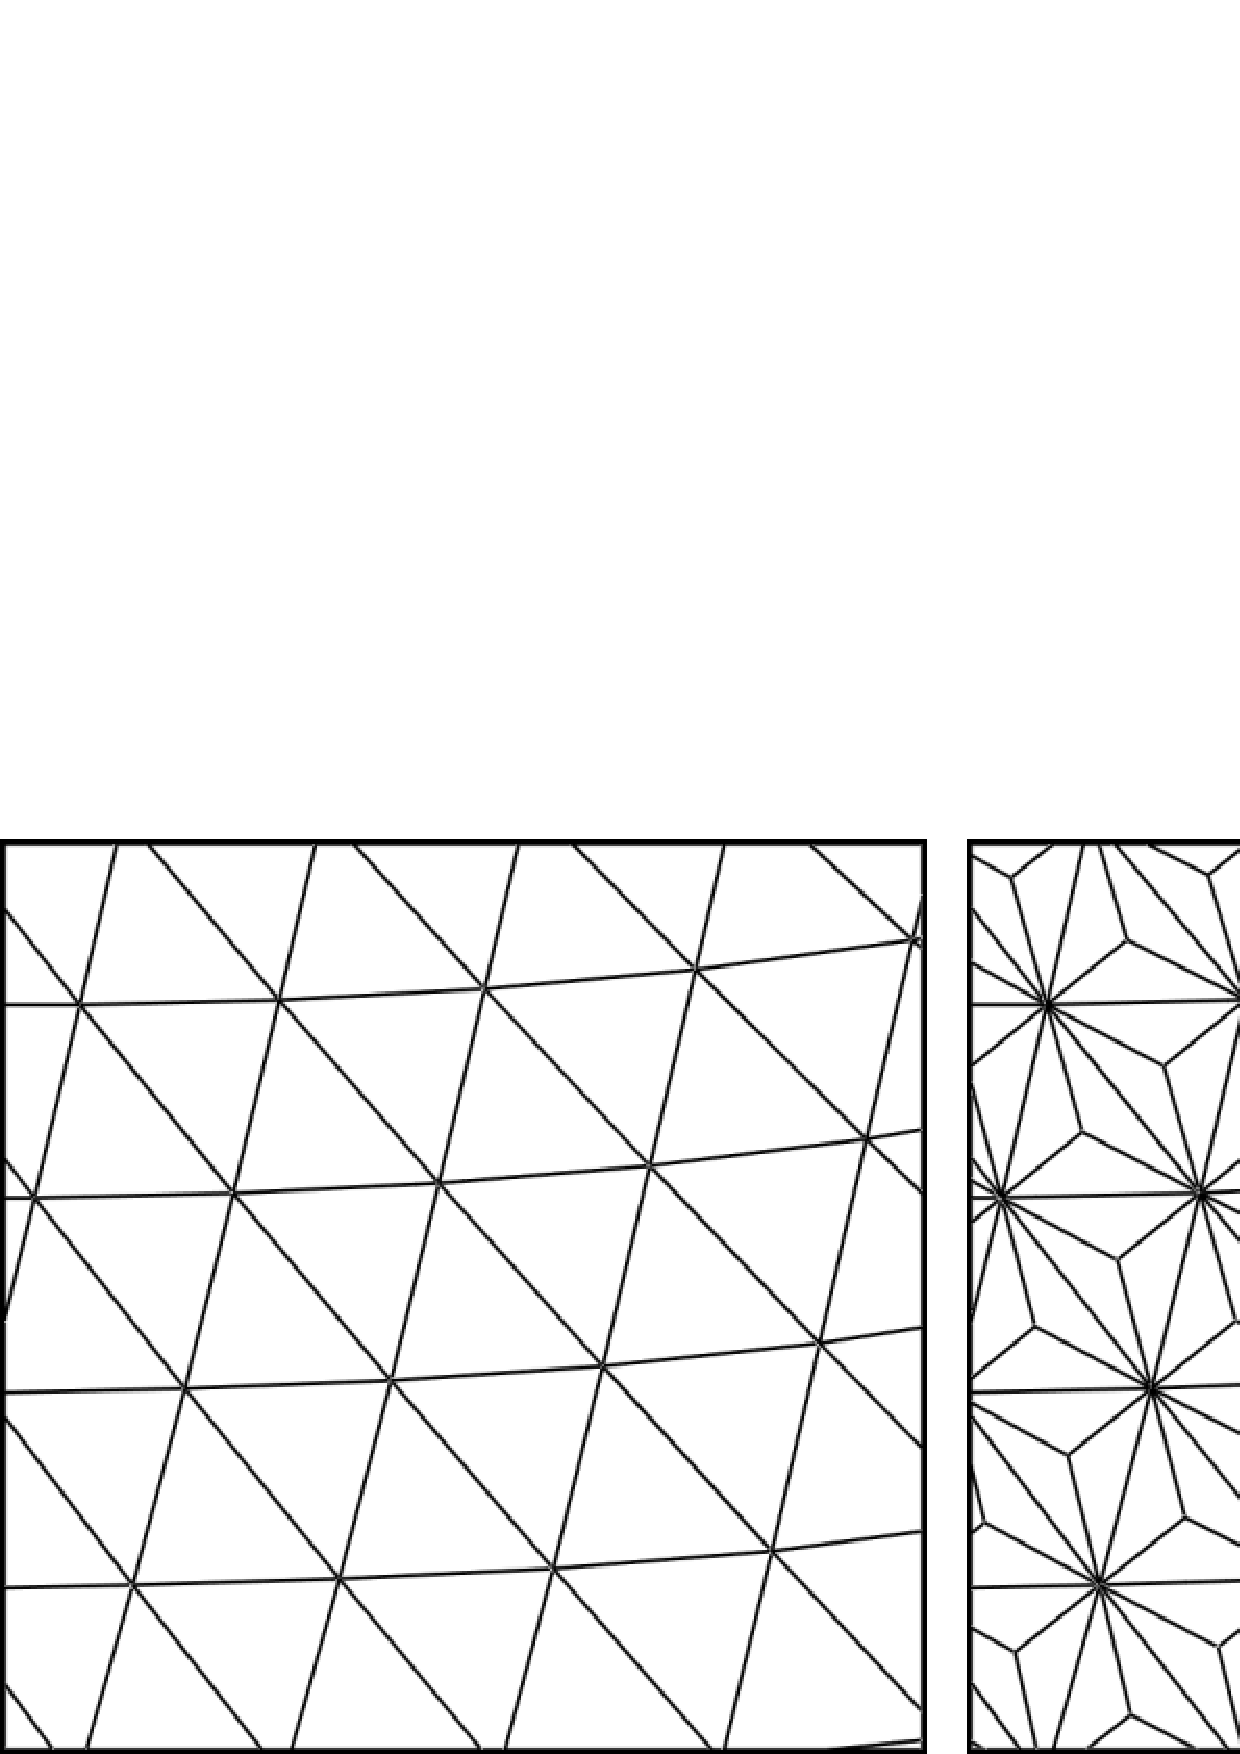
\includegraphics[width=10.0cm]{figs/sqrt3_basic}}
    \caption{The $\sqrt{3}$-Subdivision scheme is decomposed as
             a set of Euler operators: face splits and edge flips.}
    \label{fig:sqrt3_basic}
\end{figure}

The subdivision step takes a triangle mesh as input and splits each
facet at its centroid into three triangles.  We write a function that
creates the centroid for one triangle. The topology refinement part
exists already as an Euler operator in \cgalpoly, we only have to
computer the coordinates of the new vertex. Since the facet is a
triangle, we access the 1-ring of the centroid directly without any
loops or branching decisions (in general, we could use the circulator
loop shown in the render function).% in Section~\ref{sec:poly}).

% sqrt3 subdivision 

\begin{figure}[htb]
    \centering{\includegraphics[width=10.0cm]{figs/sqrt3}}
    \caption{$\sqrt{3}$ subdivision of the mannequin mesh.}
    \label{fig:sqrt3}
\end{figure}


\begin{lstlisting}
void create_centroid( Polyhedron& P, Facet_iterator f) {
  Halfedge_handle h = f->halfedge();
  Vector vec = h->vertex()->point() - ORIGIN;
  vec = vec + (h->next()->vertex()->point() - ORIGIN);
  vec = vec + (h->next()->next()->vertex()->point() - ORIGIN);
  Halfedge_handle new_center = P.create_center_vertex(h);
  new_center->vertex()->point() = ORIGIN + (vec/3.0);
}
\end{lstlisting}%\vspace*{-3mm}

\noindent
Next, all edges of the initial mesh are flipped to join two
adjacent centroids. It is part of the \cgalpoly\ interface.

Finally, each initial vertex is replaced by a barycentric combination
of its neighbors. However, the mesh has already been subdivided, so
the original neighbors of a vertex are actually every other vertex in
the 1-ring. We write a function object for the smoothing step that
can be used with the \CodeFmt{std::transform} function.

\begin{lstlisting}
struct Smooth_old_vertex {
Point operator()( const Vertex& v) const {
  std::size_t degree = v.vertex_degree()/2;
  double alpha = (4.0-2.0*cos(2.0*CGAL_PI/degree))/9.0;
  Vector vec = (v.point() - ORIGIN) * (1.0-alpha);
  Halfedge_around_vertex_const_circulator h = v.vertex_begin();
  do {
    vec = vec + ( h->opposite()->vertex()->point() - ORIGIN) 
               * alpha/degree;
    ++ h; ++ h;
  } while ( h != v.vertex_begin());
  return (ORIGIN + vec);
}};
\end{lstlisting}%\vspace*{-3mm}

\noindent
In the final subdivision program we exploit that newly created items
are appended at the end of the sequences, so that we can keep valid
iterators telling us where the old items end and where the new items
start. We are as economical as possible with the extra
storage needed in this method, which is an extra array for the
smoothed coordinates of original vertices. We start by creating the
centroids, then smooth the old vertices, and conclude with flipping
the old edges.

\begin{figure}[tb]
    \centering{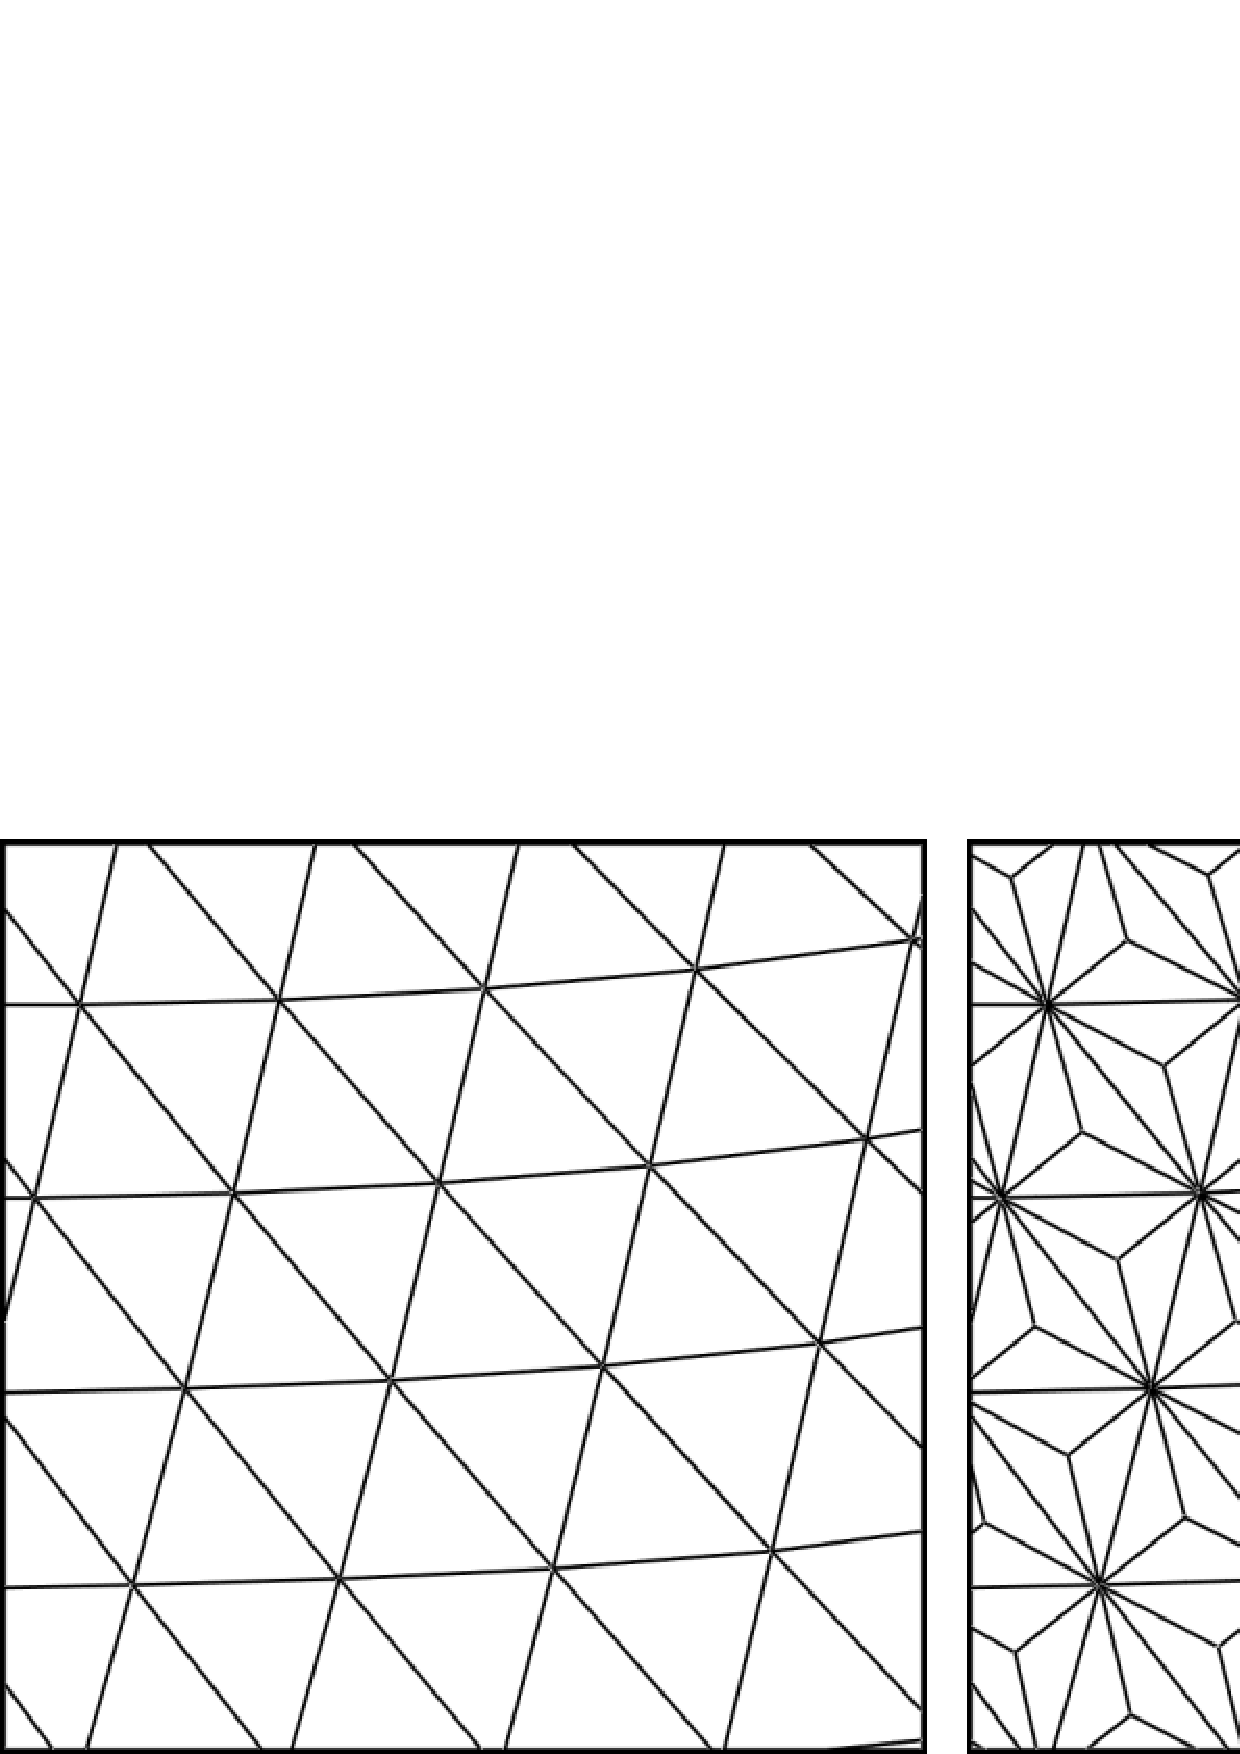
\includegraphics[width=7.0cm]{figs/sqrt3_basic}}
    \caption{The $\sqrt{3}$-subdivision scheme is decomposed into
             Euler operators: center vertex and edge flips.}
    \label{fig:sqrt3_basic}%\vspace*{-2mm}
\end{figure}


\begin{lstlisting}
void subdiv( Polyhedron& P) {
  std::size_t nv = P.size_of_vertices();
  Vertex_iterator last_v = P.vertices_end();
  --last_v;                 // the last of the old vertices
  Edge_iterator last_e = P.edges_end();
  --last_e;                 //    the last of the old edges
  Facet_iterator last_f = P.facets_end();
  --last_f;                 //   the last of the old facets
  Facet_iterator f = P.facets_begin();         // centroids
  do {
    create_centroid( P, f);
  } while ( f++ != last_f);
  std::vector<Point> pts;   //          smooth old vertices
  pts.reserve( nv);         //     space for the new points
  ++ last_v;                //   move to past-the-end again
  std::transform( P.vertices_begin(), last_v, 
            std::back_inserter( pts), Smooth_old_vertex());
  std::copy( pts.begin(), pts.end(), P.points_begin());
  ++ last_e;                //   move to past-the-end again
  for ( Edge_iterator e = P.edges_begin(); e != last_e; ++e)
    P.flip_edge(e);         //           flip the old edges
}
\end{lstlisting}%\vspace*{-3mm}

\noindent
The \openmesh\ library Release 1.0.0-beta4 comes with a demo
application for the subdivision algorithms that are available in
\openmesh. Since L.  Kobbelt, the author of the
$\sqrt{3}$-subdivision, is the head of the group developing \openmesh,
it is natural to find his algorithm in the library. We compared it
with our example implementation on a laptop with an Intel Mobile
Pentium4 running at 1.80GHz with 512KB cache and 254MB main memory
under Linux.

We selected an instance of \cgalpoly\ that was closely matching the
implementation used in \openmesh, i.e., array-storage, no plane
equation in facets, and \CodeFmt{float} coordinates in
points. \openmesh\ uses the specialized triangle-mesh data structure
where our structure remains the general polygonal mesh. We only
exploited the triangle nature of our mesh in the centroid computation,
and as it turned out, this was not crucial.  What is crucial is the
size of the structure. For example, the same experiment with an unused
plane equations in the facets increases the running time by
25\%. Similarly the choice of the coordinate type matters. We used the
lion vase, see Fig.~{fig:models} with 400k triangles as benchmark in
two successive subdivision steps. The other models had boundary edges
so that we could not use them in our currently limited example
program. Time in seconds:

\begin{center}
%\hspace*{-4mm}%
{\small
\begin{tabular}{l|ccc}
  & \multicolumn{2}{c}{{\small\cgal}} & {\small\openmesh} \\
  \textbf{$\sqrt{3}$-subdivision} & \CodeFmt{float} & \CodeFmt{double} &
  \CodeFmt{float} \\\hline
  Lion vase: step 1  & 0.95 & \hspace*{1ex}1.22 &  \hspace*{2ex}1.27 \\
  Lion vase: step 2  & 3.90 & 23.73 & 128.00
\end{tabular}
}
\end{center}

\noindent
The result is clearly encouraging for the \cgal\ implementation, but
it should be interpreted cautiously. For example, the
\openmesh\ implementation was obviously running into swap problems in
the second refinement step, which is not expected when studying the
example program and reading the manual about the default space
requirements of this implementation. Nonetheless, the simple and easy
customization possible with the \cgalpoly\ resulted in a short,
readable, and competitive implementation for this algorithm without
great efforts. It is also the first result showing that the
abstraction of Euler operations does not necessarily harm your
performance, and they clearly simplify things.

\begin{figure}
  \centering
  \epsfig{file=figs/models.eps, width=10cm}
  \caption{Models used for benchmarking.
           Complexity (in triangles):
           Bunny: 69,451,
           Lion vase: 400k,
           David (simplified version): 700k,
           Raptor: 2M.}
  \label{fig:models}%\vspace{-3mm}
\end{figure}
